\documentclass[xcolor=dvipsnames]{beamer}
\mode<presentation> {

\usecolortheme{default}
%\setbeamercovered{transparent}

\definecolor{carolina}{HTML}{82CAFA}
%\definecolor{carolina}{HTML}{3BB9FF}
%\definecolor{gray}{HTML}{B6B6B4}
%\definecolor{dark}{HTML}{151B54}

\usetheme{Madrid}
\setbeamercolor{structure}{fg=carolina}
\setbeamercolor{block title}{bg=carolina}
\setbeamercolor{block title example}{bg=carolina}

%Uncomment the following if you prefer for the font color on carolina blue background to be black.
%\setbeamercolor{block title}{fg=black,bg=carolina}
%\setbeamercolor{frametitle}{fg=black}
%\setbeamercolor{title}{fg=black}

\setbeamertemplate{caption}[numbered]
\setbeamertemplate{enumerate items}[circle]
\setbeamertemplate{itemize items}[circle]
\setbeamertemplate{section in toc}[circle]
\setcounter{tocdepth}{1} 
\setbeamercolor{section in toc}{fg=black}

\usefonttheme[onlymath]{serif}

%\setbeamertemplate{footline} % To remove the footer line in all slides uncomment this line
%\setbeamertemplate{footline}[page number] 

% To replace the footer line in all slides with a simple slide count uncomment this line
%\setbeamertemplate{navigation symbols}{}

% To remove the navigation symbols from the bottom of all slides uncomment this line
}

%some commonly used packages
\usepackage{graphics}
\usepackage{graphicx}
\usepackage{tikz}
\usepackage{fancyvrb}
\usepackage{comment}
\usepackage{amsmath}
\usepackage{amssymb}
\usepackage{lipsum}
\usepackage{subcaption}
\usepackage{caption}
\usepackage{comment}
\usepackage{multi row}
\usepackage{copyrightbox}
\usepackage{pdflscape}
\usepackage{url}
\usepackage{hyperref}

\newcommand{\overbar}[1]{\mkern 1.5mu\overline{\mkern-1.5mu#1\mkern-1.5mu}\mkern 1.5mu} %Instead of \bar or \overline, use \overbar for proper length and thickness bar for sample average. 

%Edit the following lump of code to customize with your name, title, and date
\title[Lecture 1]{BIOS 635: Introduction to Machine Learning}
\author[Kevin Donovan]{Kevin Donovan}
\institute[UNC BIOS]{UNC-Chapel Hill}
\date[1/19/2021]{1/19/2021}

\newcounter{saveenumi}
\newcommand{\seti}{\setcounter{saveenumi}{\value{enumi}}}
\newcommand{\conti}{\setcounter{enumi}{\value{saveenumi}}}

\resetcounteronoverlays{saveenumi}

\begin{document}

\begin{frame}
	\titlepage
\end{frame}

\section{Welcome}
\begin{frame}
\frametitle{\insertsectionhead}
\textbf{What is machine learning?}\\
\begin{figure}
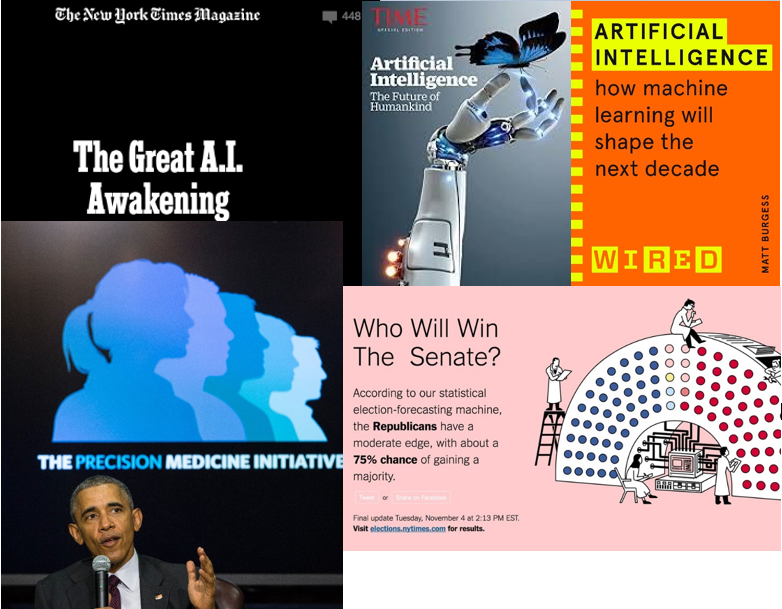
\includegraphics[scale=0.5]{images/ml_collage.png}
\end{figure}
\end{frame}

\begin{frame}
\frametitle{\insertsectionhead}
\begin{figure}

\includegraphics[scale=0.5]{images/great_power_great_resp.jpg}
\end{figure}
\end{frame}

\begin{frame}
\frametitle{\insertsectionhead}
\begin{exampleblock}{About Me}
PhD student in Biostatistics\\
UNC at Chapel Hill\\
Basketball and Green Bay Packers enthusiast\\
Hip-Hop, Jazz, Funk, Metal music fanatic
\end{exampleblock}
\end{frame}

\begin{frame}
\frametitle{\insertsectionhead}
\textbf{Structure for class}:
\begin{itemize}
\item Lecture - Tues/Thurs 9:30-10:45AM
\item Office Hours - Wed 10-11AM
\item Weekly homework assignments, bi-weekly article evaluations
\item Midterm exam on real data analysis, final group project
\item Implementation of methods taught through R
\end{itemize}

\begin{figure}
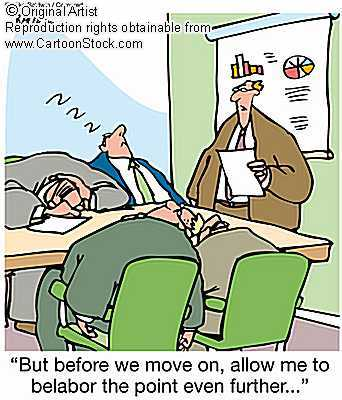
\includegraphics[scale=1.25]{images/boring-lecture.jpg}
\end{figure}

\end{frame}

\begin{frame}
\frametitle{\insertsectionhead}
\textbf{Goals for class}:
\begin{enumerate}
\item Primary: Promote the understanding of machine learning conceptually from a stats framework
\item Primary: Teach implementation of methods in R
\item Secondary: Promote good analytic practices, with focus on
\begin{enumerate}
\item data management
\item data visualization/tabulation
\item exploratory analysis
\item \textbf{reproducibility}
\end{enumerate}
\item \textbf{Develop a critical eye for machine learning and its application in science and society at large}
\end{enumerate}
\end{frame}

\section{Introduction}
\begin{frame}
\frametitle{\insertsectionhead}
\textbf{Machine Learning}:\\
Development and application of methods to identify patterns in data
\begin{figure}
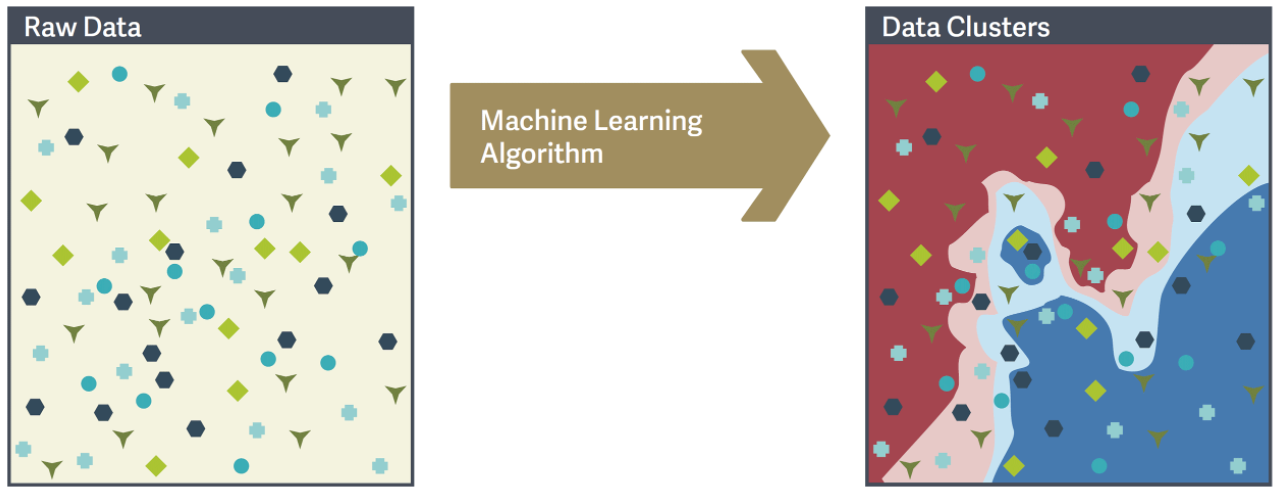
\includegraphics[scale=0.45]{images/ml_first_ex.png}
\end{figure}
\end{frame}

\begin{frame}
\frametitle{\insertsectionhead}
\textbf{How to identify these patterns?}
\begin{itemize}
\item Patterns are complex, how to model?
\item How much modeling do we enforce on the data?
\item How to evaluate a method's performance?
\item What population are we analyzing?  Who is benefiting from the analysis?  Who is being left out?
\end{itemize}
\end{frame}

\begin{frame}
\frametitle{\insertsectionhead}
\textbf{Statistical Inference}
\begin{figure}
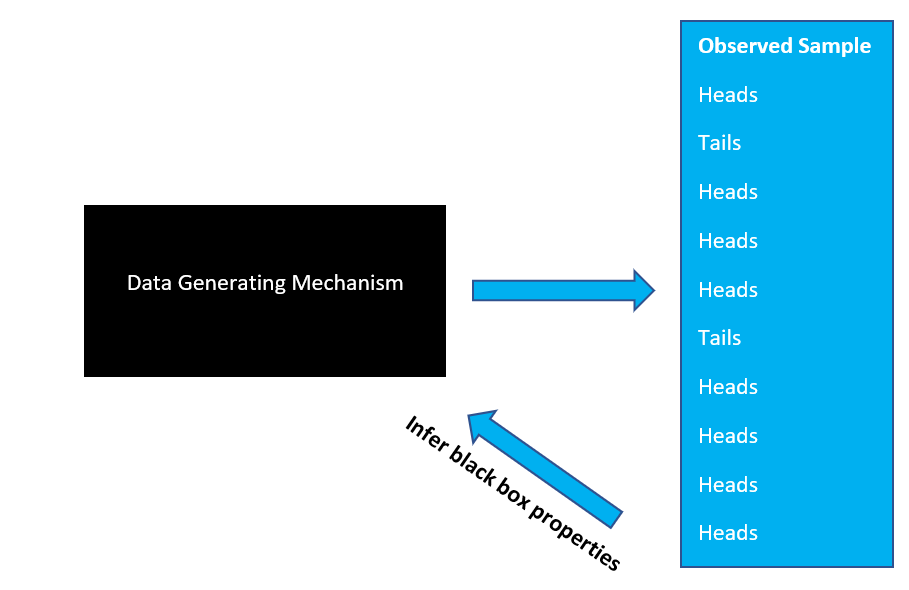
\includegraphics[scale=0.45]{images/dgm_ex.png}
\end{figure}
\textbf{Black box may be "nuisance", may only want to predict output}
\end{frame}

\begin{frame}
\frametitle{\insertsectionhead}
\textbf{Branches of machine learning}
\begin{itemize}
\item Supervised Learning\\
"Ground truth" observed for all subjects, used to "train" method
\item Unsupervised Learning\\
"Ground truth" not observed for any subjects, is "latent"
\item Reinforcement Learning\\
Algorithm "self-updates" based on data and valuation system
\end{itemize}
\end{frame}

\begin{frame}
\frametitle{\insertsectionhead}
\textbf{Supervised and Unsupervised}:\\
\textbf{Training} the method
\begin{figure}
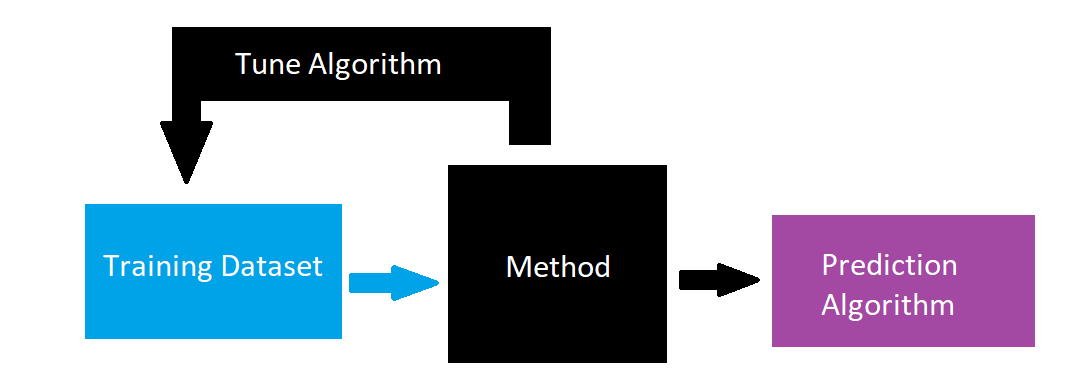
\includegraphics[scale=0.5]{images/training_diagram.png}
\end{figure}
Can we then \textbf{test} the method on the same data?\\
How training done when we \textbf{don't see the outcome}?
\end{frame}

\begin{frame}
\frametitle{\insertsectionhead}
\textbf{Supervised and Unsupervised}
\begin{figure}
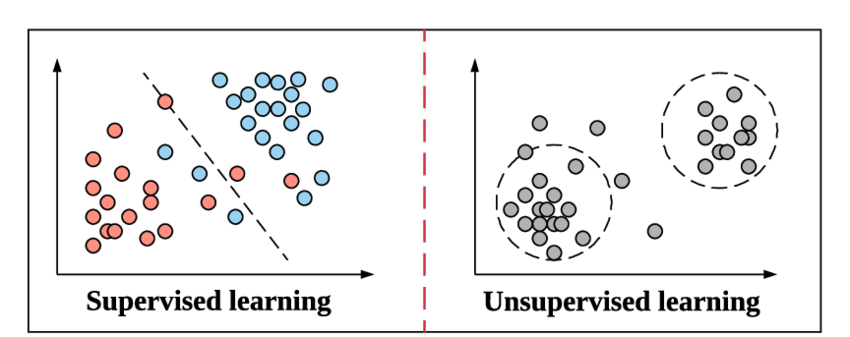
\includegraphics[scale=0.4]{images/supervised_vs_unsupervised.png}
\end{figure}
\end{frame}

\begin{frame}
\frametitle{\insertsectionhead}
Patterns found \textbf{completely dependent} on training data
\begin{itemize}
\item What population is this training data from?
\item What communities are represented, which are not?
\item Why are these communities not represented?
\item Who benefits from insights learned from method?
\end{itemize}
\begin{figure}

\includegraphics[scale=0.4]{images/nature_disparities.png}
\end{figure}
\end{frame}

\begin{frame}
\frametitle{\insertsectionhead}
\begin{itemize}
\item Many communities largely left behind in medical machine learning research
\item Reflects systemic inequities in other parts of society at large
\item As data analysts, need to combat and consider in our research
\end{itemize}
\begin{figure}

\includegraphics[scale=0.4]{images/page_cons.png}
\end{figure}
\end{frame}

\begin{frame}
\frametitle{\insertsectionhead}
\textbf{Reproducibility in the Computing Age}
\begin{figure}
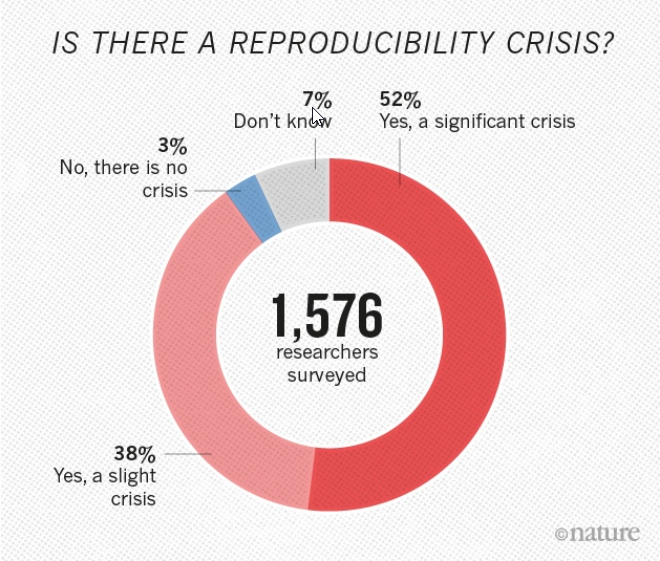
\includegraphics[scale=0.45]{images/reproducibility.png}
\end{figure}
\end{frame}

\begin{frame}
\frametitle{\insertsectionhead}
Evidence shows low reproducibility of scientific research despite
\begin{enumerate}
\item Extensive professional specialization
\item Well-developed methodology for study design and data analysis
\item Explosion in open source statistical software and computing tools
\item Software supported by extensive documentation
\end{enumerate}
\textbf{How can we turn the tide on the reproducibility issue?}
\end{frame}

\begin{frame}
\frametitle{\insertsectionhead}
\textbf{Song of the session}:\\
\href{https://www.youtube.com/watch?v=FB-DgI7wM1Y}{Pomp \& Pride by Toots and the Maytals}
\begin{figure}

\includegraphics[scale=0.5]{images/funky_kingston.jpg}
\end{figure}
\end{frame}
\end{document}

